\subsection{\newrevision{Offline MFCC Compression-Size Results}}
\label{sec:codec_results}
\begingroup
\color{green!45!black}
The team-supplied \texttt{compression.md} summarizes \nolinkurl{recording_size_comparison.csv}: 58,797 recordings, with six size observations per recording. The handoff reports no missing size values or duplicate source/path keys. The underlying CSV and optimization artifacts were not supplied with this report update, so these statistics are reproduced from the handoff rather than independently recomputed.

\begin{table}[htbp]
\centering
\color{green!45!black}
\small
\caption{\newrevision{Offline recording counts and supplied split labels.}}
\label{tab:codec_counts}
\begin{tabular}{lrrrrr}
\toprule
Source & Train & Validation & Test & Total & Int8 values \\
\midrule
Lab & 32,729 & 10,957 & 10,957 & 54,643 & 10,655,385 \\
Field & 1,434 & 427 & 2,293 & 4,154 & 810,030 \\
Total & 34,163 & 11,384 & 13,250 & 58,797 & 11,465,415 \\
\bottomrule
\end{tabular}
\end{table}

The distributions pool training, validation, and test recordings. They describe full-dataset sizes, not held-out generalization: the bank-construction process and group separation are not established by the handoff. Values exclude eight metadata bytes under the offline experiment's convention. They are not verified on-air payload lengths, and adding the current six-byte header to them would require matching the original codec and packing rules.

\begin{table}[htbp]
\centering
\color{green!45!black}
\small
\caption{\newrevision{Lab compression sizes in bytes, excluding eight metadata bytes (54,643 recordings).}}
\label{tab:codec_lab}
\begin{tabular}{lrrrrrr}
\toprule
Bank & Mean & Median & P90 & P95 & P99 & Max \\
\midrule
Balanced 2 & 46.27 & 46 & 48.0 & 49 & 51 & 68 \\
Field-only 1 & 49.19 & 49 & 51.0 & 52 & 53 & 68 \\
Field-only 2 & 47.01 & 47 & 49.0 & 50 & 51 & 69 \\
Field-only 4 & 46.40 & 46 & 49.0 & 49 & 51 & 68 \\
Field-only 8 & 46.51 & 46 & 49.0 & 49 & 51 & 68 \\
Field-only 16 & 46.64 & 47 & 49.0 & 49 & 51 & 68 \\
\bottomrule
\end{tabular}
\end{table}

\begin{table}[htbp]
\centering
\color{green!45!black}
\small
\caption{\newrevision{Field compression sizes in bytes, excluding eight metadata bytes (4,154 recordings).}}
\label{tab:codec_field}
\begin{tabular}{lrrrrrr}
\toprule
Bank & Mean & Median & P90 & P95 & P99 & Max \\
\midrule
Balanced 2 & 65.81 & 64 & 81.7 & 87 & 102 & 140 \\
Field-only 1 & 66.90 & 63 & 84.0 & 91 & 109 & 151 \\
Field-only 2 & 65.66 & 64 & 81.0 & 87 & 101 & 140 \\
Field-only 4 & 65.30 & 64 & 80.0 & 85 & 96 & 128 \\
Field-only 8 & 65.20 & 63 & 80.0 & 85 & 94 & 117 \\
Field-only 16 & 65.20 & 63 & 80.0 & 85 & 94 & 119 \\
\bottomrule
\end{tabular}
\end{table}
\FloatBarrier

\begin{figure}[htbp]
\centering
\color{green!45!black}
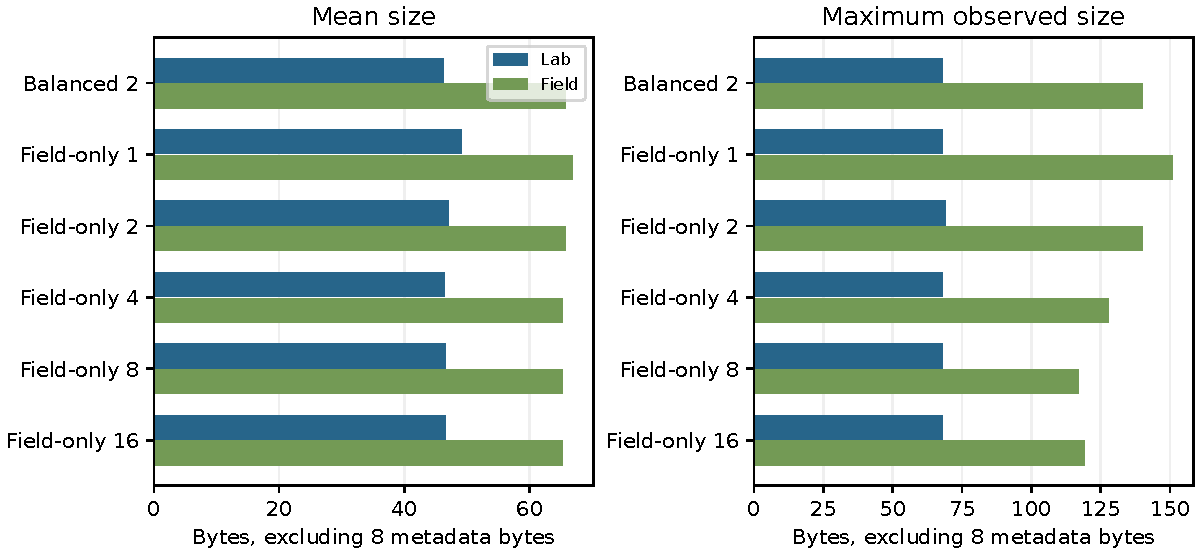
\includegraphics[width=\linewidth]{figures/compression_bank_summary.pdf}
\caption{\newrevision{Offline bank comparison reproduced from the supplied summary. Left: mean size; right: maximum observed size. Both exclude eight metadata bytes and pool all dataset splits.}}
\label{fig:codec_bank_summary}
\end{figure}
\FloatBarrier

Balanced 2 has the lowest lab mean (46.27 B); Field-only 8 averages 46.51 B. On field recordings, Field-only 8 averages 65.20 B and has a maximum of 117 B, compared with 65.81 B and 140 B for Balanced 2. Field-only 16 has the same rounded field mean but a maximum of 119 B. Field sizes are higher and more dispersed; these distributions alone do not identify a causal noise mechanism.

\begin{table}[htbp]
\centering
\color{green!45!black}
\small
\caption{\newrevision{Paired size comparison on the same recordings. Negative mean difference favors Field-only 8.}}
\label{tab:codec_paired}
\begin{tabular}{lrrrr}
\toprule
Source & Field-only 8 smaller & Equal & Balanced 2 smaller & Mean difference (B) \\
\midrule
Lab & 320 & 40,951 & 13,372 & $+0.238$ \\
Field & 1,522 & 2,082 & 550 & $-0.618$ \\
\bottomrule
\end{tabular}
\end{table}

For accounting only, an uncompressed $15\times13$ float32 matrix occupies 780 B; int8 coefficients occupy 195 B, or 199 B with a float32 scale. A hypothetical raw-int8 packet with the six-byte application header would occupy 201 B, since that header already includes the scale. These are arithmetic baselines, not additional measured CSV variants. The supplied comparison does not establish raw/int4/fixed-$k$/Huffman benchmark results, classifier accuracy, quantization error, ESP32 runtime or memory use, airtime, RF delivery, or battery savings.
\endgroup
\FloatBarrier
